% Analytic bias-versus-quadratic displacement in a constant-rate planar turn.
% The curves are evaluated directly from the continuous integral in the text.
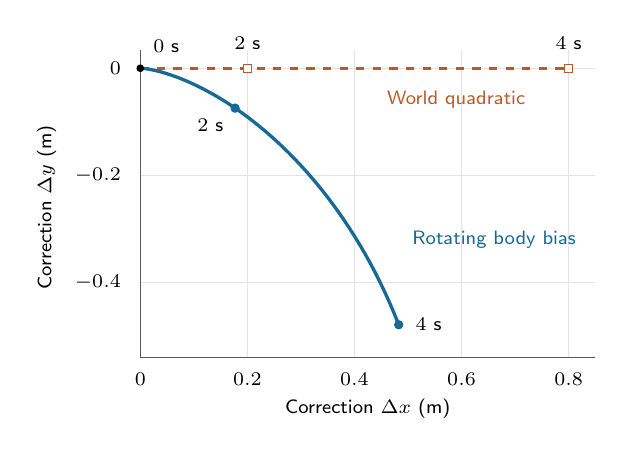
\begin{tikzpicture}[x=6.8cm,y=6.8cm,font=\sffamily\scriptsize]
  \definecolor{quadraticcolor}{RGB}{183,91,40}
  \definecolor{bodycolor}{RGB}{23,106,148}
  % Equal metric scales: these are correction displacements, not aircraft paths.
  \foreach \x in {0,.2,.4,.6,.8}{
    \draw[gray!22] (\x,-.54)--(\x,.035);
    \node[anchor=north] at (\x,-.55) {\pgfmathprintnumber[fixed,precision=1]{\x}};
  }
  \foreach \y in {-.4,-.2,0}{
    \draw[gray!22] (0,\y)--(.85,\y);
    \node[anchor=east] at (-.018,\y) {\pgfmathprintnumber[fixed,precision=1]{\y}};
  }
  \draw[black!65] (0,.035)--(0,-.54)--(.85,-.54);
  \node[rotate=90] at (-.175,-.26) {Correction $\Delta y$ (m)};
  \node[anchor=north] at (.425,-.60) {Correction $\Delta x$ (m)};
  % Endpoint acceleration is +0.10 e_x m/s^2; omega=0.60 rad/s and h=T-t.
  % q_W=a h^2 e_x/2; q_B=a[(1-cos(omega h)),sin(omega h)-omega h]/omega^2.
  \draw[quadraticcolor,very thick,dashed] (0,0)--(.8,0);
  \draw[bodycolor,very thick,domain=0:4,samples=90,variable=\h]
    plot ({.1*(1-cos(deg(.6*\h)))/.36},{.1*(sin(deg(.6*\h))-.6*\h)/.36});
  \fill[black] (0,0) circle[radius=1.4pt];
  \node[anchor=south west] at (.006,.012) {$0$ s};
  \foreach \x/\label in {.2/2,.8/4}{
    \node[draw=quadraticcolor,fill=white,inner sep=0pt,minimum size=3pt] at (\x,0) {};
    \node[anchor=south] at (\x,.017) {$\label$ s};
  }
  \fill[bodycolor] (.177123,-.074434) circle[radius=1.7pt];
  \node[anchor=north east] at (.173,-.077) {$2$ s};
  \fill[bodycolor] (.482609,-.479038) circle[radius=1.7pt];
  \node[anchor=west] at (.496,-.479) {$4$ s};
  % Direct labels and distinct marker/line styles retain monochrome legibility.
  \node[quadraticcolor,anchor=north] at (.59,-.025) {World quadratic};
  \node[bodycolor,anchor=west] at (.49,-.32) {Rotating body bias};
\end{tikzpicture}
